
科学发展的最终目的是为了解决现实问题。
为了搞明白其中的物理规律,我们从中抽象出来一个数学模型。
对于这个数学模型,如果我们有一个解析解,并且这个解析解能够很好的反映这个物理现象,
我们可以很高兴的说我们已经“解决”了或者至少“部分解决”了这个问题。
但是随着科学的发展,我们关心的问题逐渐从简单到复杂,从单一问题到多问题耦合。
在这种情况下,我们不得不做一些计算,去”逼近”这个神秘的解。
随着计算机硬件的逐渐发展,
利用计算机这个有力的工具和数学结合去解决具有实际意义的物理问题越来越显现出强大的力量。
本小节主要介绍一下算法设计中的经验与理念。

\subsection{数学转化为算法}
\begin{itemize}
\item \textbf{数学到编程:无限到有限的转换。}数学和计算机结合的关键是,
  对于一个数学问题,我们需要有一个算法的近似。
  当我们讨论一个数学对象时,我们的表示方式可能是无限维的,无穷多的。
  例如当我们讨论一个单位圆时,它的自由度是无穷多的(从点集的角度出发,它由无穷多个点构成)。
  但计算机的资源是有限的,我们不能把圆上的每个点都表示出来。
  因此我们需要将一个具有无穷维度的数学问题转化为一个能够用有限的计算机资源表示的问题。
  对于一个单位圆,我们可以用它的内接多边形或者阶梯型线段去近似它(图 \ref{fig:circle}),
  不难发现,随着多边形边数的逐渐增大,其近似程度也越来越高。
  \begin{figure}[htbp]
    \centering
    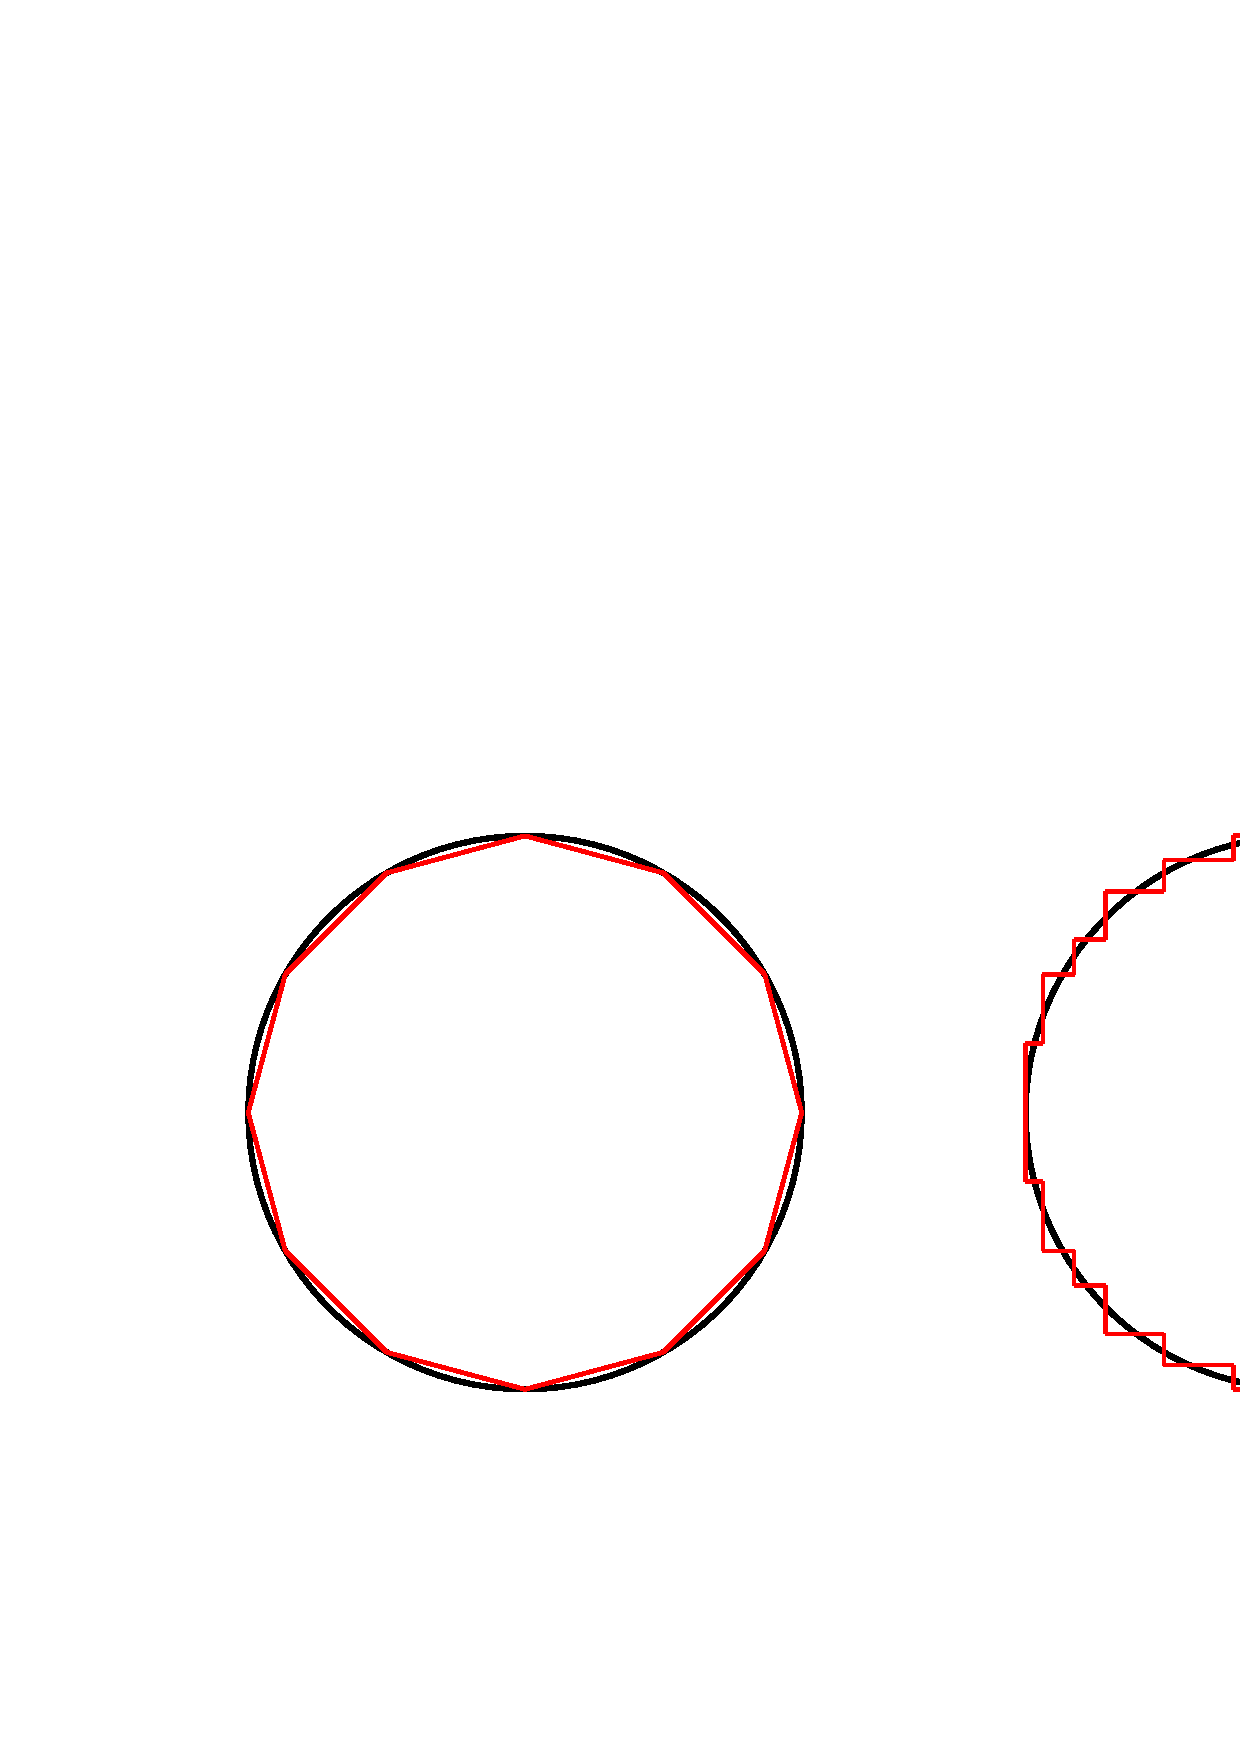
\includegraphics[width=0.40\textwidth]{eps/circle}
    \caption{ 不同图形拟合单位圆(左图为内接多边形,右图为阶梯型多边形)。\label{fig:circle}}
  \end{figure}		
\item \textbf{算法设计的原则:保证收敛,提高收敛率。}判断一个算法是否正确的原则是算法最终是否收敛。
  用$\epsilon-\delta$语言可以描述为:
  \begin{equation}
    \label{epsDel}
    \forall \epsilon >0, \;\; \exists \; N_0>0, \;\;\text{s.t.} \;\;
    \forall N > N_0, \;||E_N|| < \epsilon.
  \end{equation}
  这里,$\epsilon$ 表示想要控制的误差范围,
  $N_0$ 表示计算机资源(存储空间,运行时间等等),
  $E_N$ 表示近似模型与真实模型的误差。
  简单来说,收敛意味着想要多精确,就可以多精确,但是我们为之付出的代价可能会越来越大。
  当同一模型描述不同问题时,其收敛结果可能截然不同。
  假如我们仅仅想描述一个单位圆时,图 \ref{fig:circle} 的两种方式都可以达到目标;
  但当我们想利用近似的模型去逼近圆周长度时, 
  图 \ref{fig:circle} 右的近似方法显然是不收敛的。 
  这是因为不管用多么精细的阶梯型线段去拟合圆,其周长$l$始终满足$l \ge 8 > 2\pi$。
  另一个值得关心的概念是算法的收敛率,即一个收敛序列向其极限逼近的速度。
  在这里,我们可以看作是在相同的误差 $\epsilon$ 条件下,
  其最少投入的计算机资源 $N_0$ 的大小。$N_0$ 越小,其收敛率越高。
  而如何寻求一个合适的 $N_0$,是基于多方面因素的平衡。
\end{itemize}

\subsection{大问题到小问题的转换}
事实上,你面对的绝大多数问题往往不是你一下子就可以解决的。
在这时,学会将一个大的复杂的问题分解成小的简单的问题是一种很重要的科研能力。
虽然问题``小"的度量因人而异,但至少对你而言解决起来是相对轻松的。 
总体来说,我们应该遵循以下几个原则:
\begin{itemize}
\item \textbf{数学概念与C++类之间的简单对应。}在设计程序之前,
  请确保你已经将与程序相关的整个数学模型的概念与理论理解清楚,
  否则你会在接下来的设计中晕头转向。永远不要低估数学理论在程序设计中的重要性!
  接下来将数学中的基本概念直接映为相应的 C++ 类是一个很好的习惯, 
  这是因为在设计类时我们应遵循单一职责原则,
  即一个C++类尽量只完成一个任务或一些具有类似功能的任务。
\item \textbf{复杂类与简单类之间的交互一般放在复杂类中。}
\item \textbf{同级别类之间的交互可考虑放在一个算子类中。}
\item \textbf{每个小问题相对独立。}对问题进行分解利于我们将细节\emph{封装}(\emph{encapsulation})起来,
  这样我们就实现了将一个整体复杂度为$O(N)$的大问题转化为了若干个局部复杂度为$O(1)$的子问题。 
\end{itemize}

\subsection{关注模块的层级}
我们最后的设计中模块之间的层级关系应该如图\ref{fig:hierarchy}所示:
\begin{figure}[ht]
  \centering
  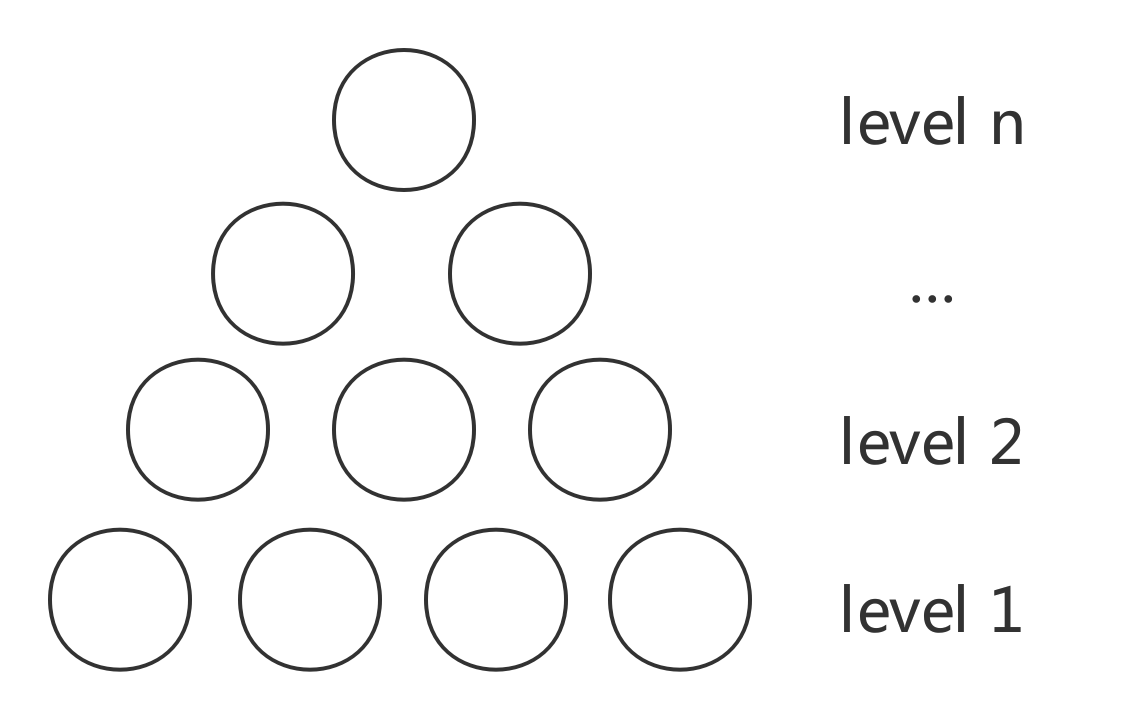
\includegraphics[width=0.30\textwidth]{png/hierarchy}
  \caption{模块间层级关系}
  \label{fig:hierarchy}
\end{figure}

其中最底层的模块主要负责将机器语言(例如某些数据结构,for循环等)
翻译成针对特定问题的语言(domain-specific language),
这里``domain" 对我们而言就是数学或者数学中一些最基本的概念。
底层的类实现机器语言和数学语言之间的转换,
使得我们的思考更集中于数学概念,而不用再考虑机器底层的细节。
在设计完成底层模块后,上层模块不宜再直接使用机器语言,
此时我们更应该从数学的角度思考问题。
正如Eckel所言:
\begin{quote}
  Create high-level abstractions to express what you're doing 
  and spend less time saying how you're doing it.
  The how has been solved once and for all and 
  is hidden in the algorithm's code, ready to be reused on demand.
\end{quote} 
在解决上层模块问题时,我们应该要牢记底层模块的契约而忘掉底层模块的具体实现细节。
底层模块与上层模块之间的关系正如学习英语时字母,单词,语句之间的关系。 
看书我们不能一个字母一个字母去看,而要一个单词一个单词去看,
学习一定时间后还需要一个句子一个句子去看。

\subsection{写好一个合格的设计文档}
整体设计完成后不要直接去写程序,先用\LaTeX{}写一个文档(\textbf{写下来!})。
其主要目的是为了确保算法设计的正确性。
在这个文档中,我们需要考虑:
\begin{itemize}
\item \textbf{整体设计的合理性。}比如:设计过程中层级是否明确?
  每个类中的成员变量是不是它的固有属性?
  算法的整体复杂度是否最小?
  重用是否发挥到最大化?
  未来需求有变化时,我们是否能够应对?等等。
\item \textbf{局部设计的规范性。}如果你已经对整体设计有一个宏观的把握, 
  已经将这个看似庞大的问题切割为一些等待解决的相互独立的小问题。
  面对这些小问题,你需要做的是:
  \begin{itemize}
  \item \emph{明确契约}
  \item \emph{设计算法}
  \item \emph{证明正确性}
  \item \emph{足够细化}
  \item \emph{写文档}
  \item \emph{程序实现}
  \item \emph{再测试}
  \end{itemize}
\end{itemize} 

\begin{remark}
在刚开始的学习阶段,我们应该严格按照上述形式进行训练。将自己的想法一步步严格写下来!
\end{remark}

\subsection{编程与调试}
编程与调试是算法设计的最后一步,而不是为了完成作业匆匆开始的第一步。
只有在熟悉整个程序设计过程,写出一份合格的设计文档后我们才开始进入编程与调试环节。
调试主要分为两种,
\begin{itemize}
\item \textbf{单一测试:}根据模块的层级,分别实现每个底层模块,
  测试这些模块,再写出这些底层模块耦合形成的模块并进行测试。 
\item \textbf{功能测试:}检查软件或者程序设计是否达到用户要求的功能。 
\end{itemize}
在有之前的准备后我们的目标应该如孙子兵法所言:不战而胜。 
好的设计,通常不需要太多时间调试!


%%% Local Variables:
%%% mode: latex
%%% TeX-master: "../Guide"
%%% End:
